%
% File eacl2009.tex
%
% Contact  oflazer@gmail.com or das@ling.uni-potsdam.de
%%

%% Based on the style files for EACL 2006 by 
%%e.agirre@ehu.es or Sergi.Balari@uab.es
%% and that of ACL 08 by Joakim Nivre and Noah Smith

\documentclass[11pt]{article}
\usepackage{eacl2009}
\usepackage{times}
\usepackage{url}
\usepackage{polski}
\usepackage[T1]{fontenc}
\usepackage[utf8]{inputenc}
\usepackage{latexsym}
\usepackage{listings}
\usepackage{graphicx}
\usepackage{float}
\usepackage{color}
%\setlength\titlebox{6.5cm}    % You can expand the title box if you
% really have to

\title{Spejd Web Service}

\author{Szymon Acedański\\
  Uniwersytet Warszawski\\
  {\tt accek@mimuw.edu.pl}}
\date{2009-11-21}

\newcommand{\todo}[1]{\textcolor{red}{
    {\tiny\sffamily{}T\hspace{-1pt}O\hspace{-1pt}D\hspace{-1pt}O} #1}}

\newcommand{\fn}[1]{\texttt{#1}}
\newcommand{\param}[1]{\textit{#1}}
\newcommand{\tag}[1]{\textsc{#1}}

\begin{document}
\maketitle
\begin{abstract}
W~artykule opisano Web Service służący do powierzchniowego parsowania tekstów
przy pomocy Spejda~--- narzędzia do tego celu opracowanego w~IPI PAN
polskiego opracowanego w~IPI PAN. Przeniesienie Spejda w~świat internetu ma służyć
przede wszystkim ułatwieniu korzystania z~niego przez jak najwięcej osób.
Dlatego w~tej pracy skupiono się na opisie usługi od strony użytkownika,
przedstawieniu możliwości i~sposobu użycia.

Spejd Web Service od wersji 3 wykorzystuje do oznaczania wprowadzonego czystego
tekstu tagger TaKIPI \cite{takipi} przy pomocy dostarczonego Web Service'u
\cite{takipiws}.

\end{abstract}

\section{Wstęp}

Spejd \cite{spejd} to narzędzie do powierzchniowego przetwarzania tekstów oraz do
dezambiguacji morfosyntaktycznej. Został opracowany w~IPI PAN w~2007 roku
w~ramach prac nad projektem Narodowego Korpusu Języka Polskiego. 

Stworzenie Web Servicu do tego programu ma na celu ułatwienie
korzystania z~niego jak największej rzeszy użytkowników. Ma również zachęcić
do tworzenia łatwo dostępnych, bo opartych na technologii internetu, serwisów
pokrewnych, udostępniając prosty i~przejrzysty interfejs programistyczny. 
Wykorzystanie web servicu eliminuje również nakład pracy związany z~koniecznością
dołączania i~utrzymywania Spejda przez autorów (względnie użytkowników)
programów, które z~niego korzystają.

Niejako przy okazji powstały również dwie dodatkowe rzeczy:
\begin{itemize}
  \item prosta strona internetowa pod nazwą \emph{iSpejd}, przez którą można
    interaktywnie korzystać z~systemu~--- wystarczy wprowadzić zestaw reguł oraz
    tekst (można też wybrać reguły bądź teksty z~listy predefiniowanych), żeby
    w~przeglądarce zobaczyć efekt przetwarzania,
  \item skrypt i~usługa służące do konwersji dokumentów z~formatu IPI PAN do
    HTMLa.
\end{itemize}

W kolejnych częściach pracy opisuję pokrótce sposób korzystania z usługi Spejd
Web Service oraz strony iSpejd.

\section{Dostęp do usługi Spejd}

Do komunikacji z~usługą sieciową Spejda używany jest protokół XML\dywiz RPC
\cite{xmlrpc}. Usługa działa pod adresem
\url{http://spejdws.appspot.com/xmlrpc}. Dokładny opis składni zapytań oraz
sposobu ich wysyłania znajduje się w~specyfikacji wspomnianego protokołu.

Usługa Spejd Web Service udostępnia następujące operacje:
\begin{itemize}
  \item \fn{string getVersion()}

    Zwraca napis zawierający numer wersji usługi.

  \item \fn{list<string> listPredefinedRuleSets()}

    Zwraca listę nazw predefiniowanych zestawów reguł zapisanych w~systemie.
    
    Można ich użyć w~operacji \fn{parse} przekazując jako parametr
    \param{rulesMode} napis \texttt{PREDEFINED}, a~nazwę reguły jako parametr
    \param{rules}.

  \item \fn{string getPredefinedRuleSet(\\string name)}

    Zwraca reguły z~predefiniowanego zestawu o~wskazanej nazwie. Są zwracane
    jako pojedynczy napis (zazwyczaj zawierający wiele linii) w~języku Spejda.

  \item \fn{list<string> listPredefinedTexts()}

    Zwraca listę nazw predefiniowanych tekstów.

    Można ich użyć w~operacji \fn{parse} przekazując jako parametr
    \param{textMode} napis \texttt{PREDEFINED}, a~nazwę tekstu jako parametr
    \param{text}.

  \item \fn{string getPredefinedText(\\string name)}

    Zwraca predefiniowany tekst o~danej nazwie. Jest on zwracany jako dokument
    XML w~formacie IPI PAN.

    Modyfikacja predefiniowanych zestawów reguł oraz tekstów wymaga interwencji
    operatora. Jest opisana w~pliku \texttt{README} w~dystrybucji serwisu.

  \item \fn{string parse(string rulesMode, string textMode, String rules, string text)}

    Parsuje podany tekst za pomocą podanych reguł i~zwraca wynik
    jako dokument XML w~formacie IPI PAN.

    Jeśli jako \param{rulesMode} przekazano napis \texttt{PREDEFINED},
    wtedy w~parametrze \param{rules} należy przekazać nazwę predefiniowanego
    zestawu reguł. Jeśli się chce użyć własnych reguł, należy jako
    parametr \param{rulesMode} przekazać wartość \texttt{CUSTOM}.

    Podobnie parametr \param{textMode} może przyjąć wartość \texttt{PREDEFINED}
    jeśli chce się użyć gotowego tekstu. Jeśli chce się podać własny tekst
    w~formacie IPI PAN, należy podać wartość \texttt{XML}. Usługa akceptuje
    również zwykły tekst. Wtedy należy podać \texttt{PLAIN}.
    
    Istnieje też możliwość przepuszczenia dostarczonego czystego tekstu przez
    tager morfosyntaktyczny TaKIPI przed przekazaniem do Spejda. W~tym przypadku
    jako \param{testMode} należy przekazać \texttt{PLAIN-TO-TAG}.
    
    Czysty tekst nie jest przetwarzany analizatorem morfosyntaktycznym. Jest
    poddawany prostej segmentacji: granice zdań wyznaczają kropki, a~segmentów
    wyrazy. Wyrazom przypisywany jest jeden możliwy tag~--- \tag{ign}.
    Znaki przestankowe są traktowane jako osobne segmenty otagowane jako
    \tag{interp}.
    
    Do przetwarzania tekstów wykorzystana jest domyślna konfiguracja Spejda oraz
    domyślna konfiguracja tagsetu, odpowiadająca tagsetowi IPI PAN \cite{tagset}
    z~dodanymi dwoma specjalnymi klasami gramatycznymi: \tag{liczba} oraz
    \tag{waluta}.
    

\end{itemize}

\noindent Od wersji 1.1 usługa udostępnia jeszcze dwie funkcje, dzięki którym
można jej użyć do konwersji dowolnych tekstów w~formacie IPI PAN do eleganckiego
HTMLa. 

\begin{itemize}
  \item \fn{string formatXmlAsHtml(\\string xml)}

    Konwertuje przekazany dokument z~formatu IPI PAN do formatu HTML.
    Zwraca fragment zgodny ze standardem HTMLa. Warto zwrócić uwagę, że zwrócony
    dokument nie jest sam w~sobie poprawnym dokumentem HTML, lecz jedynie jego
    fragmentem, który należy umieścić wewnątrz elementu \texttt{<body>}.

    Aby poprawnie wyświetlić zwrócony fragment, następujący plik CSS musi
    zostać dołączony do dokumentu:
    \url{http://spejdws.appspot.com/css/ipipanxces.css}.
    
    Wygodny skrypt, którego można użyć z~linii komend do wyświetlania
    tekstów sformatowanych tym sposobem, znajduje się w~dystrybucji w~katalogu
    \texttt{extras}. Nazywa się \texttt{ipipan2html.py}.

  \item \fn{string parseAndFormatAsHtml(\\
    string rulesMode, \\
    string textMode, \\
    string rules, string text)}

    Ta funkcja jest po prostu połączeniem dwóch powyższych. Parsuje podany tekst
    za pomocą wybranych reguł oraz zwraca wynik w~formacie HTML.
\end{itemize}

\textbf{
Przy wywoływaniu powyższych metod przez XML-RPC, ich nazwy należy poprzedzić
prefiksem ,,\texttt{SpejdService.}''.} Listing~\ref{lst:req} pokazuje przykładowe
zapytanie. Metodą \fn{parse} przetwarzany jest tekst ,,Jest
2000 rok.'' przy użyciu jednej reguły, która ustawia tag wszystkich liczb na
\tag{liczba} oraz tworzy z nich jednoelementowe grupy składniowe.

\clearpage
\lstset{language=XML, caption=Przykład zapytania XML-RPC, label=lst:req}
\begin{lstlisting}[frame=trbl]
POST /xmlrpc HTTP/1.0
Host: spejdws.appspot.com
User-Agent: xmlrpclib.py/1.0.1
    (by www.pythonware.com)
Content-Type: text/xml
Content-Length: 433

<?xml version='1.0'?>
<methodCall>
<methodName>SpejdService.parse
  </methodName>
<params>
<param>
<value>
<string>CUSTOM</string>
</value>
</param>
<param>
<value>
<string>PLAIN</string>
</value>
</param>
<param>
<value><string>
Rule "liczby"
Match: [orth~"[0-9]*"];
Eval: set(liczba,"liczba",1);
      group("LICZBA",1,1);
</string></value>
</param>
<param>
<value><string>Jest 2000 rok.
  </string></value>
</param>
</params>
</methodCall>
\end{lstlisting} 

\section{\emph{iSpejd}~--- interaktywny Spejd}

iSpejd jest prostym serwisem WWW, przez który każdy może spróbować swoich sił
w~przetwarzaniu powierzchniowym. Jest dostępny na stronie
\url{http://spejdws.appspot.com}. Po wpisaniu tego adresu w~przeglądarce
pojawia się formularz, w~którym można wpisać bądź wybrać z~listy zarówno zestaw
reguł Spejda, jak również tekst do przetwarzania. Na rysunku~\ref{fig:ispejd}
przedstawiono wygląd strony z~pokazanym wynikiem parsowania.

Strona jest dostępna w~dwóch językach -- polskim i~angielskim.

\lstset{language=XML, caption=Odpowiedź serwera XML-RPC, label=lst:resp}
\begin{lstlisting}[frame=trbl]
HTTP/1.0 200 OK
Content-Type: text/xml
Date: Mon, 07 Sep 2009
  04:16:57 GMT
Server: Google Frontend
Cache-Control: private,
  x-gzip-ok=""

<?xml version="1.0"
  encoding="UTF-8"?>
<methodResponse xmlns:ex=
  "http://ws.apache.org/xmlrpc
  /namespaces/extensions">
<params><param><value>

[ entity-escaped response here ]

</value>
</param></params>
</methodResponse>
\end{lstlisting} 

\begin{figure*}[htb]
  \begin{center}
    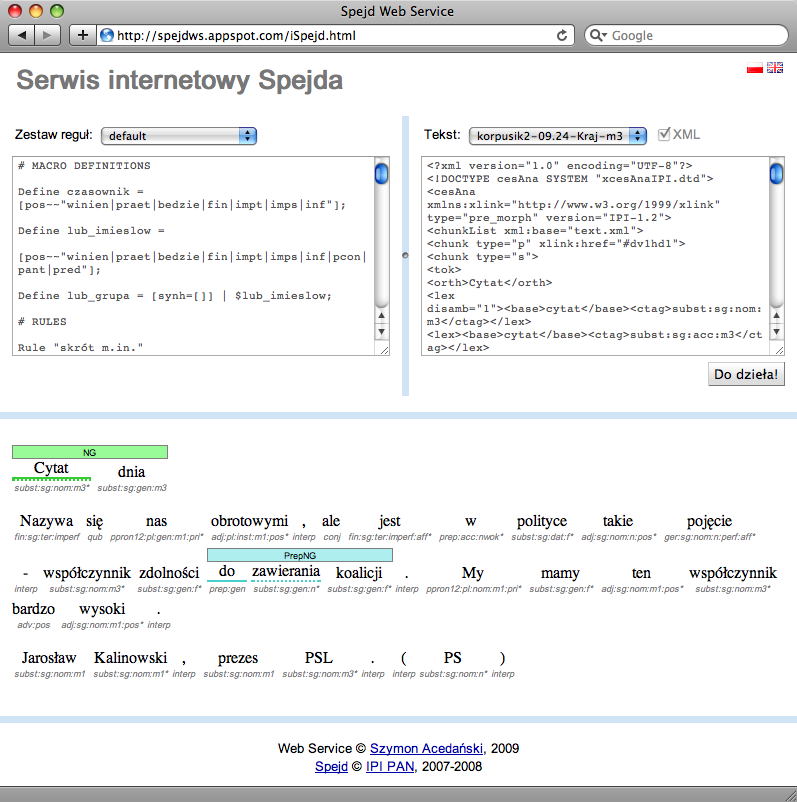
\includegraphics[width=\textwidth]{ispejd}
  \end{center}
  \caption{Strona iSpejda}
  \label{fig:ispejd}
\end{figure*}

\section{Informacje techniczne}

Zarówno Web Service, jak i~iSpejd, zostały uruchomione przy użyciu
infrastruktury Google App Engine~\cite{appengine}. Google udostępnia wszystkim
swoim użytkownikom możliwość umieszczania na serwerach aplikacji internetowych.
Usługa jest darmowa, o~ile nie przekracza się niemałych w~sumie dziennych limitów
określających dopuszczalną liczbę zapytań, zużycie procesora oraz dysku itp.

Web Service został wykonany przy użyciu technologii Java
Servlets~\cite{servlets}. Do przetwarzania zapytań XML\dywiz RPC wykorzystana
została bibliotekę \emph{ws\dywiz xmlrpc}~\cite{wsxmlrpc}.
Strona iSpejd została wykonana przy użyciu biblioteki Google Web Toolkit
\cite{gwt}.

\section{Podsumowanie}

Przedstawiony w~pracy system pozwala szerokiej gamie osób zainteresowanych
przetwarzaniem języka polskiego, na prosty dostęp do parsera powierzchniowego
Spejd. Może być także pomocą w~prowadzeniu zajęć edukacyjnych i~popularyzacji
dyscyplin związanych z~przetwarzaniem języka naturalnego.

Poniżej przedstawiam kilka pomysłów na dalszy rozwój serwisu.
\begin{itemize}
  \item integracja modyfikacji Spejda wykonanych na potrzeby projektu 
    z~kodem autora,
  \item automatyczna ewaluacja gramatyki przy danym korpusie wzorcowym,
  \item parsowanie fragmentów korpusu IPI PAN wybieranych zapytaniami Morfeusza.
\end{itemize}

\noindent \textbf{System można pobrać ze strony
\url{http://www.mimuw.edu.pl/~accek/spejdws/}.}

\bibliographystyle{acl}
% you bib file should really go here
\bibliography{eacl2009}

\end{document}

% vim:tw=80
